\subsection{Transfer particle velocities to grid}

The first thing we need to do after advecting the particles is to transfer the particle velocities to our velocity field. To do this, we are going to use the barycentric coordinates of a particle inside a cell to decide how much of the velocity of the particle is going to affect the neighboring velocities on the MAC grid. Since velocities $u$ and $v$ are stored on different axes on the MAC grid, we need to be careful when we weight and transfer the particle velocities. The easy case would be when the particle position $\vec{x}_p$ is aligned exactly at the middle of the edge between two cells. Let's compare the difference between $u$ and $v$. 

\begin{figure}[ht!]
\centering
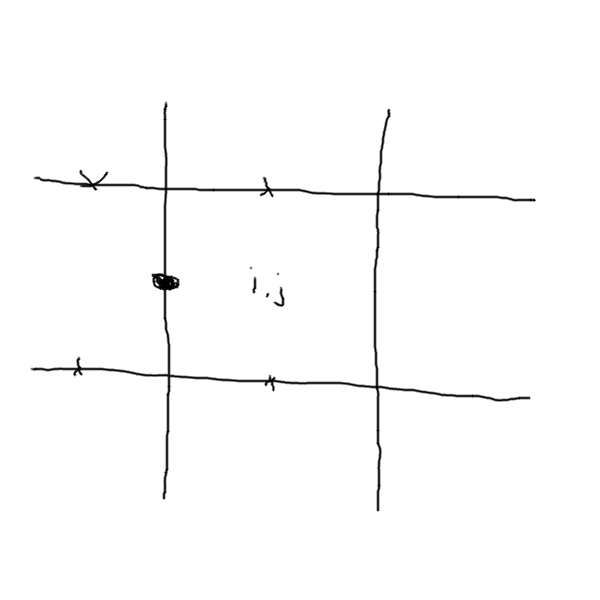
\includegraphics[width=80mm]{ch3/onedge.png}
\caption{A simple caption}
\label{onedge}
\end{figure}

In Figure \ref{onedge} the particle position $\vec{x}_p$ is exactly at grid position $(i-1/2,j)$. It is reasonable that the horizontal component of the velocity of the particle, $u_p$ only affects the MAC grid at $u_{i-1/2,j}$. The vertical component, $v_p$ is not exactly aligned with an vertical edge. This is where the barycentric coordinates come handy. As can seen, the position $\vec{x}_p$ is exactly in the middle of the rectangle that the vertical edges $v_{i-1,j-1/2}, v_{i,j-1/2}, v_{i-1,j+1/2}, v_{i,j+1/2} $ is creating. In this case, it makes sense that the vertical component of the particle velocity $v_p$ should affect the velocity field at all four edges and since it it's in the middle of the rectangle the particle velocity should affect the edges equally much.

\begin{figure}[ht!]
\centering
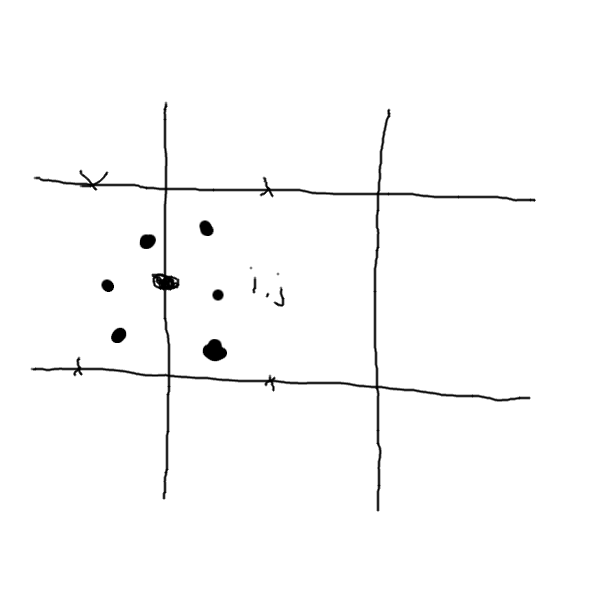
\includegraphics[width=80mm]{ch3/fouredge.png}
\caption{A simple caption}
\label{fouredge}
\end{figure}

What if there are multiple particles, how do they all affect the velocities in the grid together? As can be seen in Figure \ref{fouredge}, there are definitely going to be cases where mutiple particles are going to affect a single velocity in the MAC grid. We need a way to weight the velocities so that particle velocities closer to an edge have more effect than the ones further away. The final velocity of an edge on the MAC grid is decided by

\begin{eqnarray}
u_{i-1/2,j} = \frac{\sum\limits_{i\in A}\omega_i(x_i) u_{i}}{\sum\limits_{i \in A}\omega_i(x_i)} \\
v_{i,j-1/2} = \frac{ \sum\limits_{i \in B}\lambda_i(x_i) v_{i}}{\sum\limits_{i \in B}\lambda_i(x_i)}
\label{weightsums}
\end{eqnarray}

where $A$ is the set of particles around the horizontal edges and $\omega(x_i)$ is the horizontal weighting function. $B$ is then the set of particles around the vertical edges and $\lambda(x_i)$ is the vertical weighting function.

\begin{figure}[ht!]
\centering
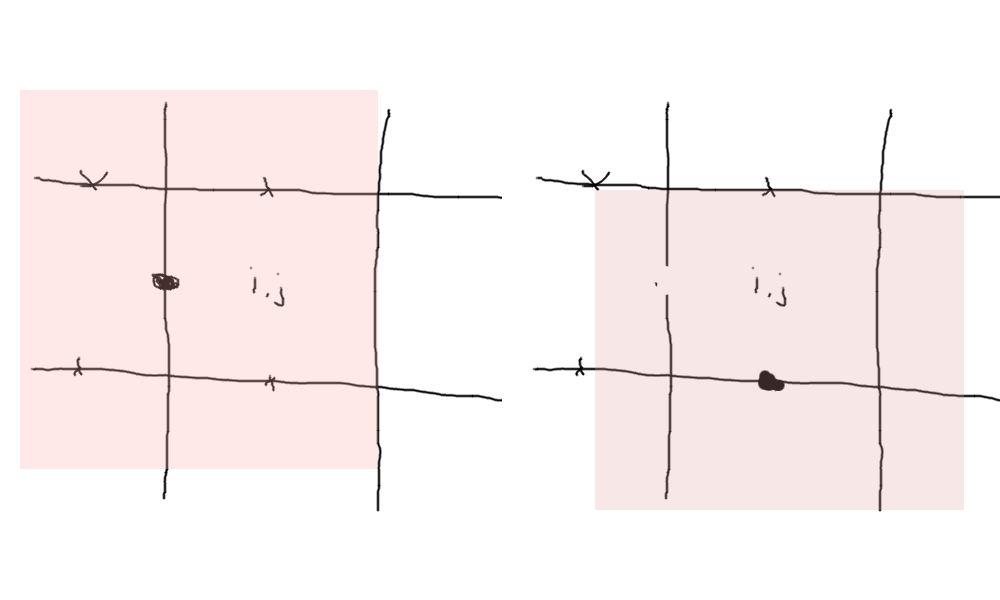
\includegraphics[width=80mm]{ch3/areaA.png}
\caption{A simple caption}
\label{areaa}
\end{figure}

Figure \ref{areaa} shows the difference between $A$ and $B$. Updating one edge at a time would require a sophisticated way of only quering particles close to the edge. This would require us to come up with a complicted data structure to store our particles to avoid $O(n)$ time complexity when gather sets $A$ and $B$ for each edge where $n$ is the total number of particles in the simulation. Instead, we will use a technique called splatting. In splatting approaches, one iterate over all the particles instead of the grid. Then for each particle, find out which edges it could possible affect, which is fast since each particle has a position and $A$ and $B$ have a fixed maximum size. The splatting part is divided into two parts. Part one can be seen in Algorithm \ref{particlestogridalgorithm1}. Notice that there is a temporary $sum$ MAC grid for storing the denominator part of Equation \ref{weightsums}.

\begin{algorithm}
\caption{Step one in splatting particle velocities to grid velocities}
\begin{algorithmic}
\STATE grid = empty mac grid
\STATE sum = empty mac grid
\FOR{all particles $p$}
\STATE tx,ty = barycentricA(p.x)
\FOR{neighboring horizontal edges $e$}
\STATE weight = omega(tx,ty, p.x)
\STATE grid.u[e.idx] += weight * p.u
\STATE sum.u[e.idx] += weight
\ENDFOR
\STATE tx,ty = barycentricB(p.x)
\FOR{neighboring vertical edges $e$}
\STATE weight = lambda(tx,ty, p.x)
\STATE grid.v[e.idx] += weight * p.v
\STATE sum.v[e.idx] += weight
\ENDFOR
\ENDFOR
\end{algorithmic}
\label{particlestogridalgorithm1}
\end{algorithm}

The barycentric functions in Algorithm \ref{particlestogridalgorithm1} returns two normalized coordinates from $0$ to $1$ where bottom left of the region gives back $(0,0$, bottom right $(1,0$, top left $(0,1)$ and top right $(1,1)$. Anything inbetween gets linearly interpolated.

\begin{algorithm}
\caption{Step two in splatting particle velocities to grid velocities}
\begin{algorithmic}
\FOR{$i=0$ to $N_x$}
\FOR{$j=0$ to $N_y$}
\STATE idx = .... get index for (i-1/2,j)
\STATE grid.u[idx] /= sum.u[idx]
\STATE idx = ... get index for (i,j-1/2)
\STATE grid.v[idx] /= sum.v[idx]
\ENDFOR
\ENDFOR
\end{algorithmic}
\label{particlestogridalgorithm2}
\end{algorithm}

The second step of the splatting process is to normalize all the velocities. In Algorithm \ref{particlestogridalgorithm1} we only applied the numerator of Equation \ref{weightsums}. Once all velocities are splatted we have the sum of all weights for every edge. Next step is  to devide the current edge velocity with the sum stored at each edge and the transfer is done.
